\documentclass[a4paper,12pt]{article}
%minimal: Este tipo de documento sólo permite establecer el tamaño de la página y la fuente. Documentos MUY cortos
%proc: Documentos más cortos
%article: Documentos cortos
%report: Documentos medio largos
%book: Hacer libros(Capítulos, apéndices)
%memoir: Todo en 1
%Más fuentes en 
%https://community.rstudio.com/t/cant-creat-pdf-cant-find-tinytex-or-miktex-files/34960
%https://tug.org/FontCatalogue/mathfonts.html

%12pt: Tamaño de letra de 12 puntos
%twocolumns: Doble columna
\usepackage{ 
comment,        %Para hacer comentarios largos
graphicx,       %Para meter figuritas
enumitem,       %Para hacer listas chidas (Paquete esencial en la vida)
amsfonts,       %Las letras de pizarra
amsmath,        %Fracciones, integrales y otras cosas
amsthm,         %Teoremas
amssymb,        %Más símbolos
mathtools,      %MÁS SÍMBOLOS
mathrsfs,       %Letras cursivas matemáticas
bm,             %Letras matemáticas negritas
bbm,            %Esta da la indicadora con \mathbbm 1
physics,        %Símbolos físicos
chronology,     %Líneas de tiempo
tikz,           %Figuras
pgfplots        %Gráficas
}
\usepackage[ruled,vlined,spanish,onelanguage]{algorithm2e} %Algoritmos
\usepackage[utf8]{inputenc}
% Para que el documento pueda poner acentos y demás caracteres.
\title{La tarea que pidió Imanol} %Aquí va el título
\author{Pues yo, quién más}  %El autor
\date{Hoy} %La fecha

\newcommand{\RR}{\mathbb{R}}

\setlength\parindent{0pt}
%Quitar sangría
\begin{document}
\maketitle %Aquí pedimos que se ponga el título, autor y fecha
añ 

\begin{abstract}
	En este documento vamos a aprender a usar \LaTeX (\TeX).
\end{abstract}


A en unicode (U+0041). \textbf{Así ponemos las letras negritas}. \emph{Así las itálicas} o \textit{así}. \underline{Así subrayamos cosas}. \textbf{\underline{llll}}.\\
\section{Lista del súper}
\begin{itemize}
\item[$\square$] Zanahorias, 
\item[c)] Aguacate,
\item Manzanas,
\item Naranjas,
\item $\frac{1}{2}$kg de fresas, %Así se ponen las fracciones chiquitas dentro del texto
\item $\dfrac{1}{4}$kg queso parmesano.%Así se ponen las fracciones grandes dentro del texto
\end{itemize}

\section{Pasos para superar el alcoholismo}
\begin{enumerate}
\item Aceptar que tienes un problema.
\item Ir a tomar café con @ImanolBuscaTag.
\end{enumerate}

\subsection{Lista del súper}
\begin{itemize}[label=$\square$]
\item Zanahorias, 
\item Aguacate,
\item Manzanas,
\item Naranjas,
\item $\frac{1}{2}$kg de fresas, %Así se ponen las fracciones chiquitas dentro del texto
\item $\dfrac{1}{4}$kg queso parmesano.%Así se ponen las fracciones grandes dentro del texto
\end{itemize}

%\part{}  Éste no sirve para archivos tipo article
%\chapter{} Éste tampoco
%\section{}
%\subsection{}
%\subsubsection{}
%\paragraph{}    No lo vamos a ocupar
%\subparagraph{}     Tampoco


A + ` = À

?`% Así se pone el caracter ¿

\'a %Poner acento
\\ %Salto de línea
Sea $f:[a,b]\to\mathbb R$ una función continua y $F:[a,b]\to\mathbb R$ una función tal que $F'(x)=f(x),$ para toda $x\in [a,b]$, entonces
\[\dv[n]{f}{x}  \]
\[3.14^2\pdv[2]{u}{x} =  \pdv[2]{u}{t}\]



efeaxwqx

\begin{algorithm}[h]
\KwData{$n$ un número natural.}
\KwResult{ El \begin{math}n\end{math}-ésimo término de la sucesión de Fibonacci.}
$aux=n$\,
\If{aux = 0,1}{
regresa 1
}{
Fibonacci($aux-1$)+Fibonacci($aux-2$)
}
\caption{Fibonacci}
\end{algorithm}


\begin{algorithm}
 \KwData{Una matriz $C$ de costos.}
 \KwResult{$\overline U$ conjunto inicial de asignaciones,\\ $\varphi$ un inicial vector de asignación de personas,\\ $f$ un vector inicial de asignación de tareas,\\$(u,v)$ una solución dual factible.}
  \For{$i \in\{1,...,n\}$}{
   $u_i := \min\{c_{i,j}:j\in\{1,...,n\}\}$\;
   }
  \For{$j \in\{1,...,n\}$}{
   $v_j := \min\{c_{i,j}-u_i : i\in\{1,...,n\}\}$
   }
  \For{$i \in\{1,...,n\}$}{
   \For{$j \in\{1,...,n\}$}{
    \If{$f(j) = 0$, $c_{i,j}-u_i-v_j=0$ y $i\notin\overline U$ }{
    $f(j) = i$\;
    $\varphi(i) = j$\;
    $\overline U = \overline U \cup \{i\}$
    }
   }
  }
 \caption{Preprocesamiento}
\end{algorithm}


5tef
erger

\begin{comment}
A ver David, aquí debes de poner tu parte de la tarea
¡¡¡Aquí!!!
¡¡¡AQUÍ!!!
\end{comment}

\# \$ \% \^{} \& \_ $\{$ $\}$ \~{} $\backslash$



\begin{itemize}
\item 10pt, 11pt, 12pt,... : Cambiar el tamaño de la fuente.
\item a4paper, letterpaper, legalpaper: Tamaño del papel.
\item fleqn: Pasar las fórmulas del centro a la izquierda.
\item leqno: números de izquerda a derecha.
\item titlepage, notitlepage: para poner o no poner una sola página con título.
\item twocolumn, onecolumn: para poner el documento con dos columnas o una columna.
\item twoside, oneside: Documento de dos caras o una cara(article o report).
\item landscape: Para que el documento esté en forma horizontal.
\item openright, openany: Para que el nuevo capítulo (de un documento tipo Book) empiece del lado derecho o empiece en cualquier lado.
\end{itemize}

\[\left| \det \begin{pmatrix}
3 & 2 & 0\\
4 & 10 & 10\\
4 & 9 & 10
\end{pmatrix}\right|
\]

\[\bordermatrix{ & 1 & 2 \cr 
1 & 1/2 & 1/2 \cr 
2 & 1/2 & 1/2 \cr }\]

\[\begin{bmatrix}
3 & 2 & 0\\
4 & 10 & 10\\
4 & 9 & 10
\end{bmatrix}
\]

\[\begin{Bmatrix}
3 & 2 & 0\\
4 & 10 & 10\\
4 & 9 & 10
\end{Bmatrix}
\]

\[\begin{vmatrix}
3 & 2 & 0\\
4 & 10 & 10\\
4 & 9 & 10
\end{vmatrix}
\]

\[\Bigg(\begin{matrix}
3 & 2 & 0\\
4 & 10 & 10\\
4 & 9 & 10
\end{matrix}\Bigg)
\]

\[\mathbb E \left[Y_{t+1} \Bigg| \sum_{i=1}^{N_t}Y_i\right] \]

\[\int_a^b x dx = \frac{x^2}{2}\bigg|_{x=a}^{x=b}\]

\[f(x) = \begin{cases}
 \lambda e^{-\lambda x} & \text{si }x>0,\\
 0 & \text{e.o.c.}
 \end{cases}
\]

\[\text{frfrf }\int_a^b f\]

Quiero meter matrices al texto $\mathcal{E}leospapie$$\begin{pmatrix}
3 & 2 & 0\\
4 & 10 & 10\\
4 & 9 & 10
\end{pmatrix}$, esto se va a ver feo :'(. $\left(\begin{smallmatrix}
3 & 2 & 0\\
4 & 10 & 10\\
\end{smallmatrix}\right)$\\ 


Definimos a la función $f:[0,1]\to \RR$ dada por $f(x) = x^2/(x+5)$. La gráfica de $f$ es la siguiente
\begin{figure}
\centering
\begin{tikzpicture}
\begin{axis}[
title = La persona corriendo,
axis lines = left,
xlabel = {Time [h]},
ylabel = {Distance [m]},
xmin = 0,
xmax = 1,
ymin = 0,
ymax = 1,
xtick distance=10^(-1),
ytick distance=10^(-1),
legend pos = north east,
ymajorgrids = true,
xmajorgrids = true,
grid style = dashed,
]
\addplot[
domain = 0:1,
samples = 100,
color = magenta,
]{x^2/(x+5)+0.5};
\addplot[
color = cyan,
mark = square,
]
coordinates{(0.5,0.5)(0.6,0.6)};

\legend{eee,op};
\end{axis}
\end{tikzpicture}
\end{figure}


\[
\begin{cases}
\dot y_1&= 5y_1y_2-y_1\\
\dot y_2&= 3y_1-y_2
\end{cases}
\]

\begin{figure}
\centering
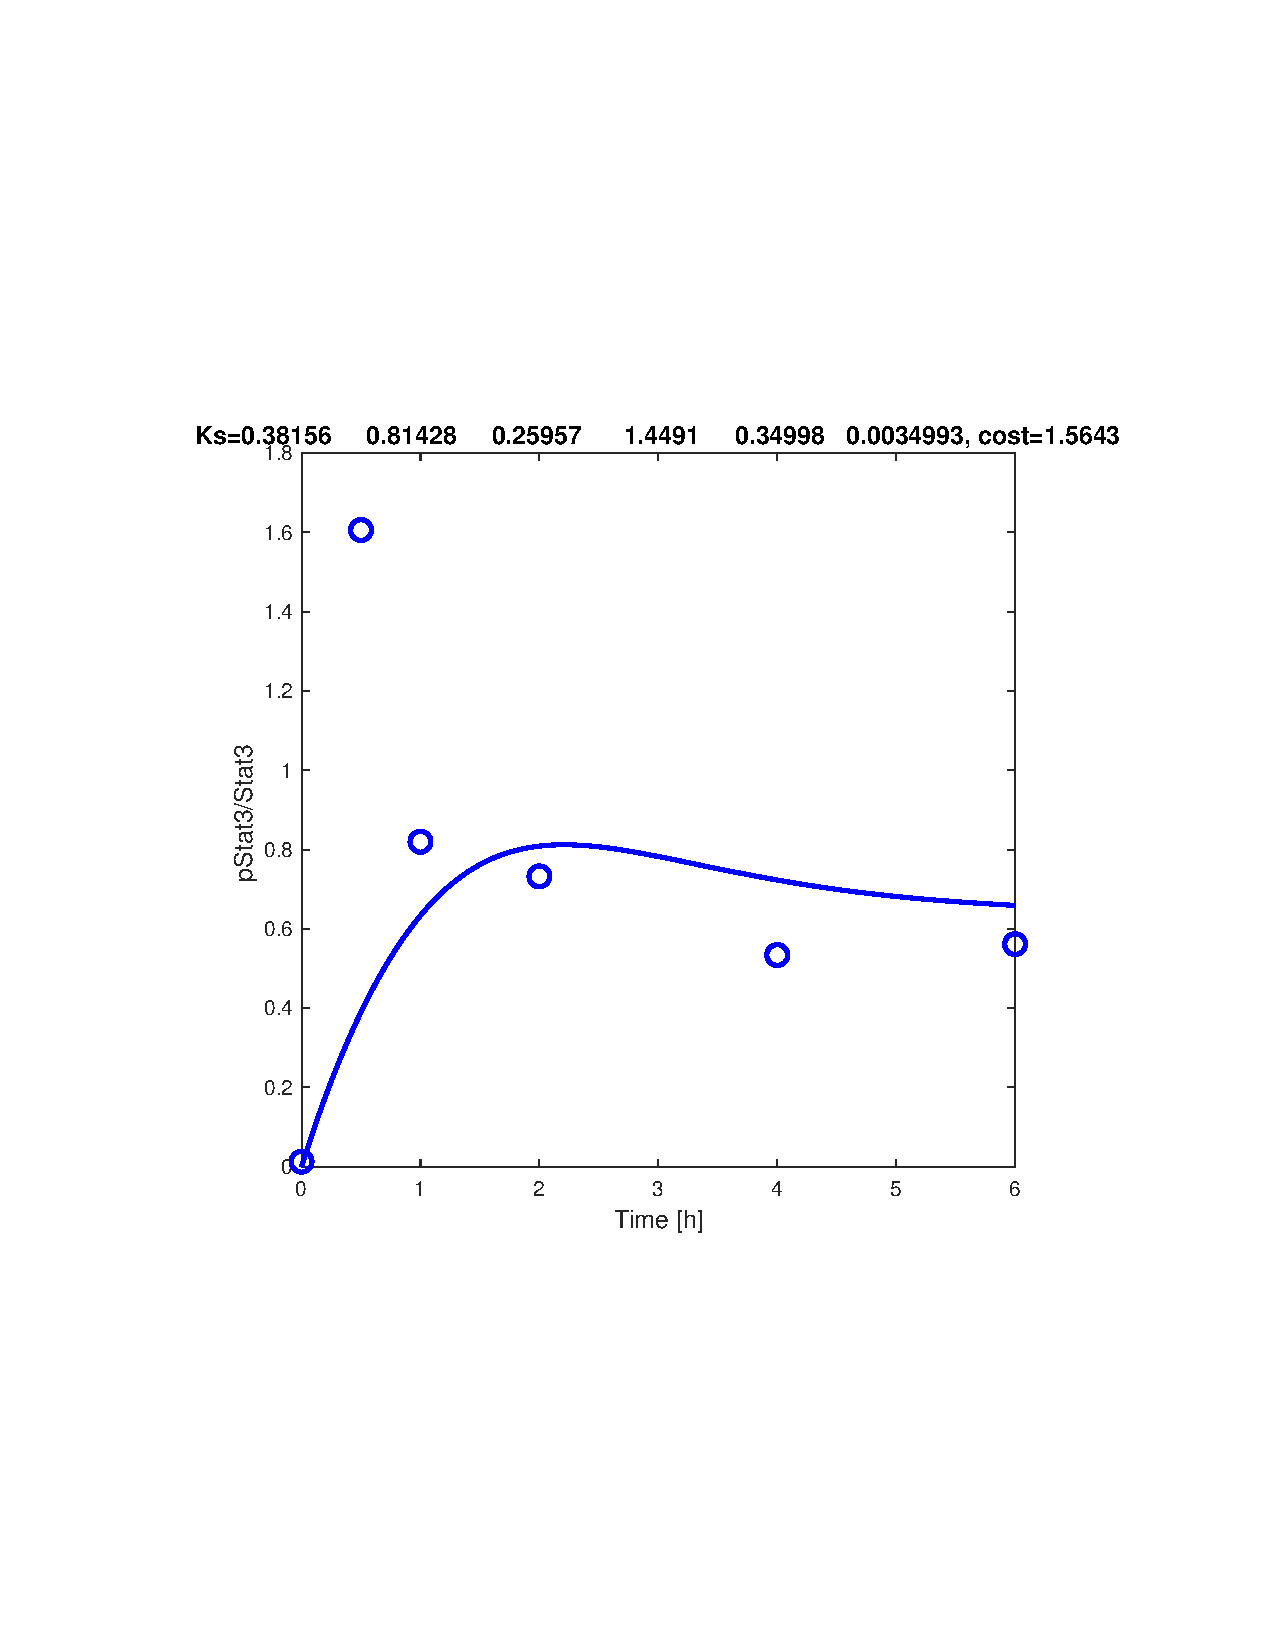
\includegraphics[width = 0.9\textwidth,trim =  {0 7.5cm 0 7.5 cm}, clip]{mifigura.pdf}
\caption{Gráfica de ode45}
\end{figure}





\end{document}